%GiG
\documentclass{beamer} 
\usetheme{Copenhagen}
\setbeamertemplate{navigation symbols}{}
\setbeamertemplate{headline}{}
\DeclareMathOperator*{\argmax}{arg\,max}

\usepackage{hyperref}


\definecolor{azure}{rgb}{0.0, 0.5, 1.0}
%\newcommand{\tblue}[1]{\textcolor{blue}{#1}}
\newcommand{\tblue}[1]{{\Large {\textcolor{azure}{#1}}}}
\newcommand{\thblue}[1]{{\Huge {\textcolor{azure}{#1}}}}
\newcommand{\hred}[1]{{\textcolor{red}{#1}}}
\newcommand{\furl}[1]{{\footnote{\url{#1}}}}

\newcommand{\mypause}{\pause}
%\newcommand{\mypause}{}

\title[Saravanan Thirumuruganathan] 
{Lecture 10: Neural Networks and Deep Learning}

\author[CSE 5334, Data Mining] 
{Instructor: Saravanan Thirumuruganathan}

\date[] 

\begin{document}


\begin{frame}
  \titlepage
\end{frame}

%\begin{frame}{Outline}
%  \tableofcontents
%  % You might wish to add the option [pausesections]
%\end{frame}

\section{Outline}

\begin{frame}
\frametitle {Outline}
    \begin{enumerate}
        \item Perceptron
        \item Neural Networks
        \item Deep Learning
    \end{enumerate}
\end{frame}


%\begin{frame}{In-Class Quizzes}
%\begin{itemize}
%\item {\Large {\bf URL:}} {\LARGE \bf \url{http://m.socrative.com/}} 
%\item {\Large {\bf Room Name:} {\LARGE \bf 4f2bb99e}}
%\end{itemize}
%\end{frame}


\section{Neural Networks}
\begin{frame}{} 
    \begin{center}
        \thblue{Neural Networks}
    \end{center}
\end{frame}

\begin{frame}{Brains\furl{http://pages.cs.wisc.edu/~jerryzhu/cs540/handouts/neural.pdf}}
    \begin{center}
        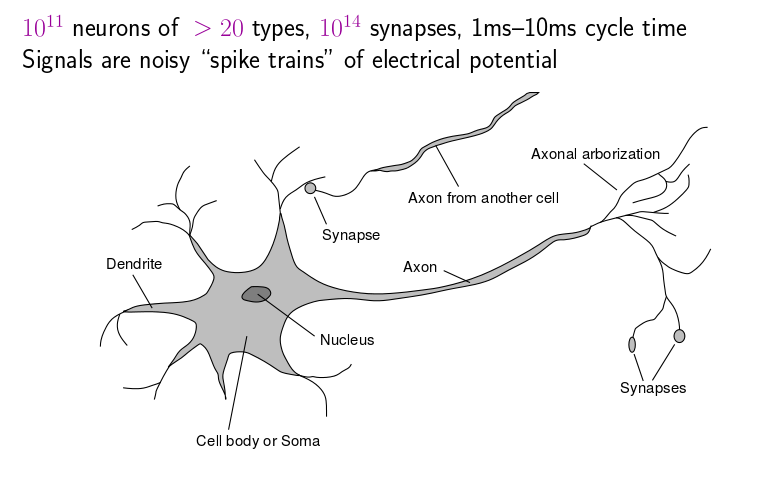
\includegraphics[scale=0.4]{brains.png}
    \end{center}
\end{frame}
\begin{frame}{SkyNet\furl{http://pages.cs.wisc.edu/~jerryzhu/cs540/handouts/neural.pdf}}
    \begin{center}
        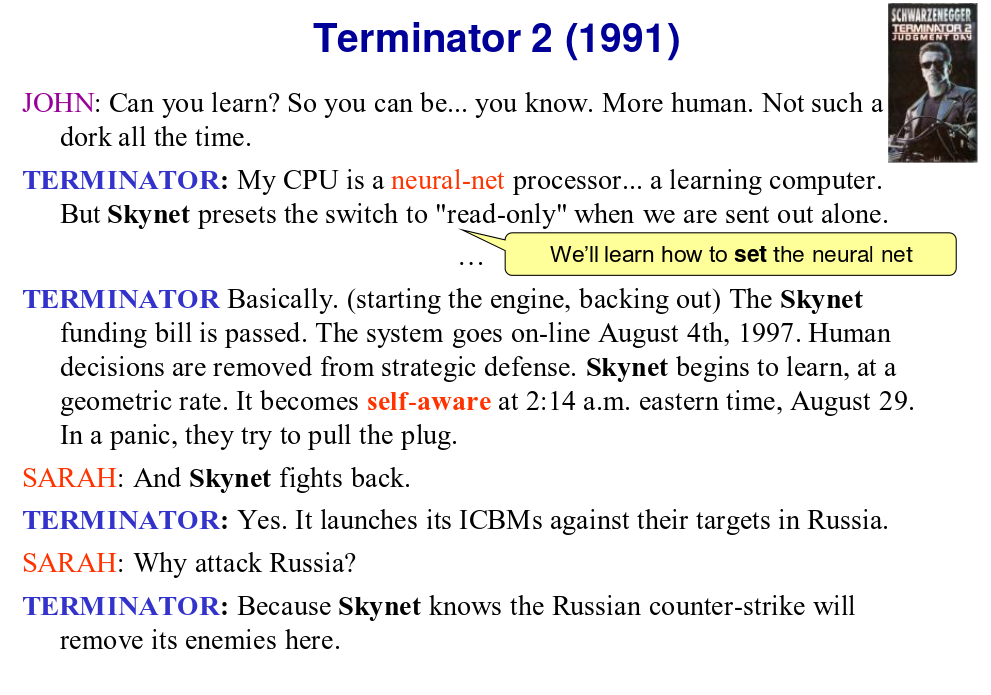
\includegraphics[scale=0.3]{skynet.png}
    \end{center}
\end{frame}

\begin{frame}{Perceptron}
    \begin{center}
        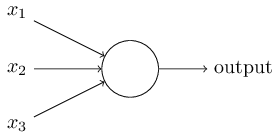
\includegraphics[scale=0.4]{perceptron.png}
    \end{center}
\end{frame}
\begin{frame}{}
    \begin{center}
        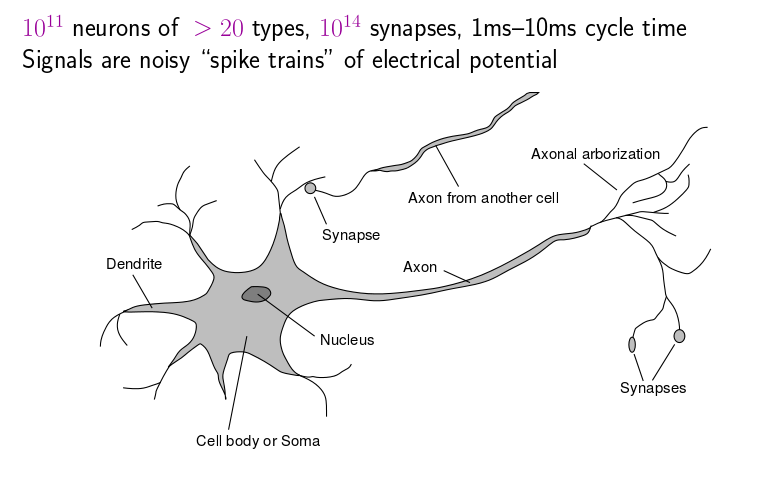
\includegraphics[scale=0.4]{brains.png}
    \end{center}
\end{frame}
\begin{frame}{}
    \begin{center}
        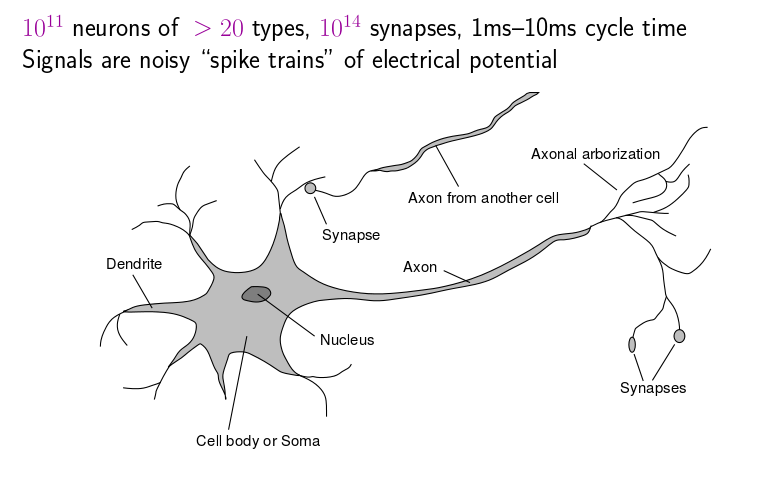
\includegraphics[scale=0.4]{brains.png}
    \end{center}
\end{frame}
\begin{frame}{}
    \begin{center}
        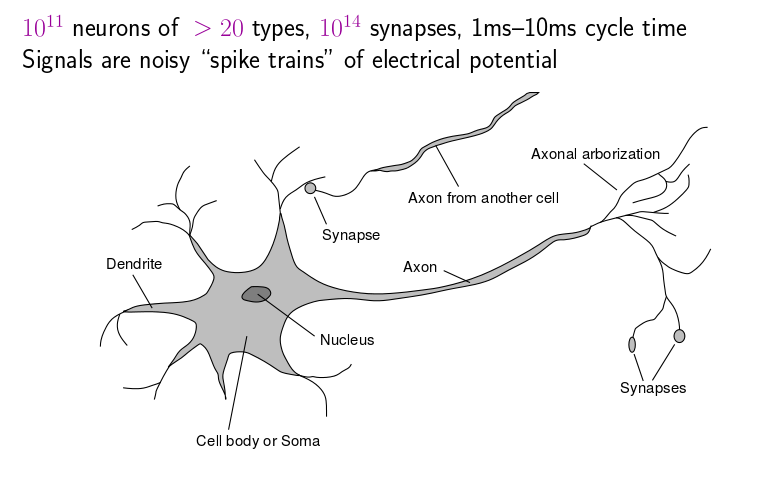
\includegraphics[scale=0.4]{brains.png}
    \end{center}
\end{frame}
\begin{frame}{}
    \begin{center}
        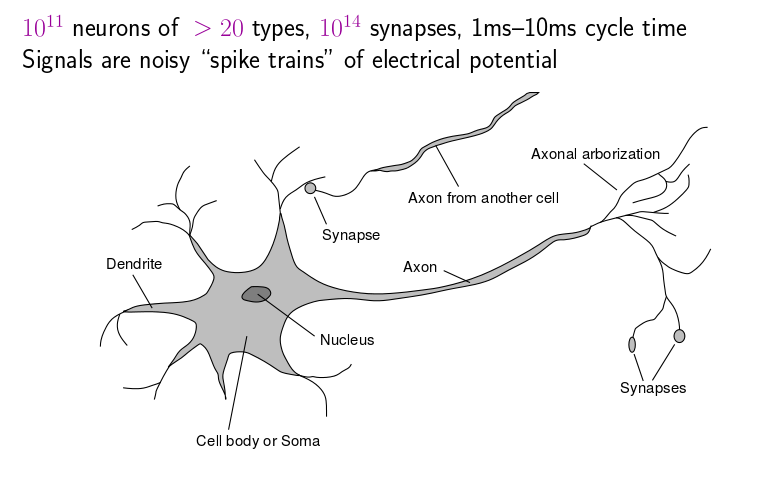
\includegraphics[scale=0.4]{brains.png}
    \end{center}
\end{frame}
\begin{frame}{}
    \begin{center}
        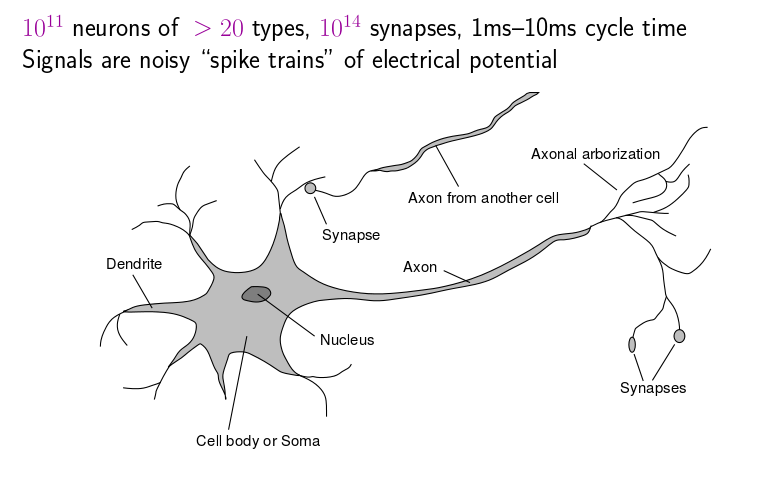
\includegraphics[scale=0.4]{brains.png}
    \end{center}
\end{frame}
\begin{frame}{}
    \begin{center}
        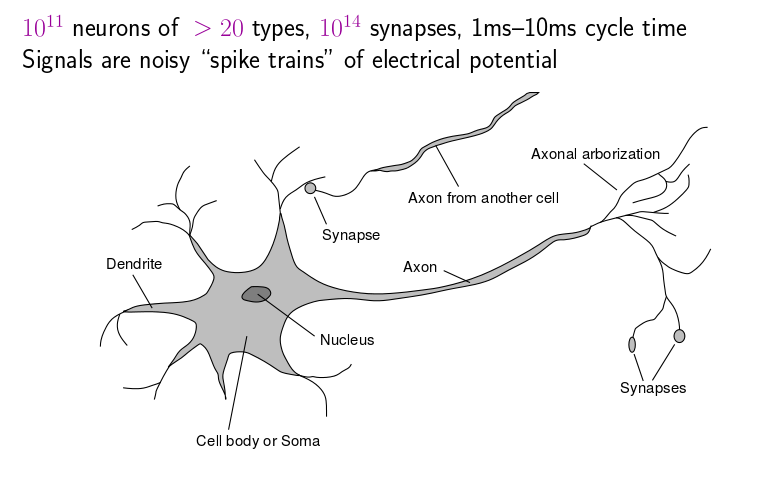
\includegraphics[scale=0.4]{brains.png}
    \end{center}
\end{frame}
\begin{frame}{}
    \begin{center}
        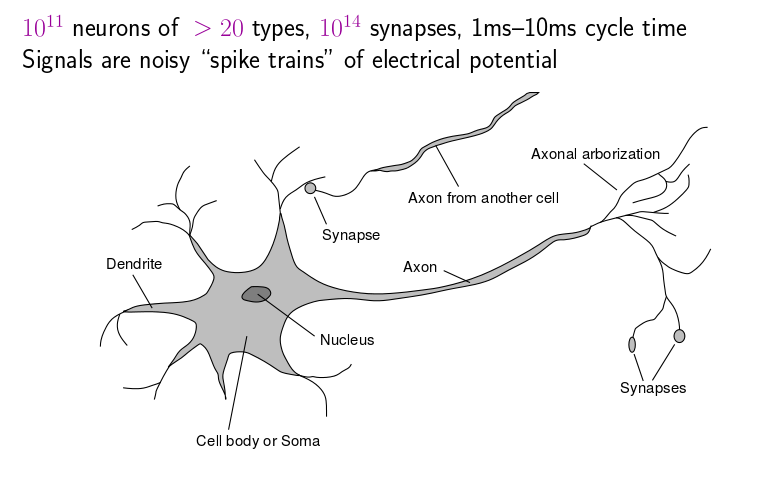
\includegraphics[scale=0.4]{brains.png}
    \end{center}
\end{frame}
\begin{frame}{}
    \begin{center}
        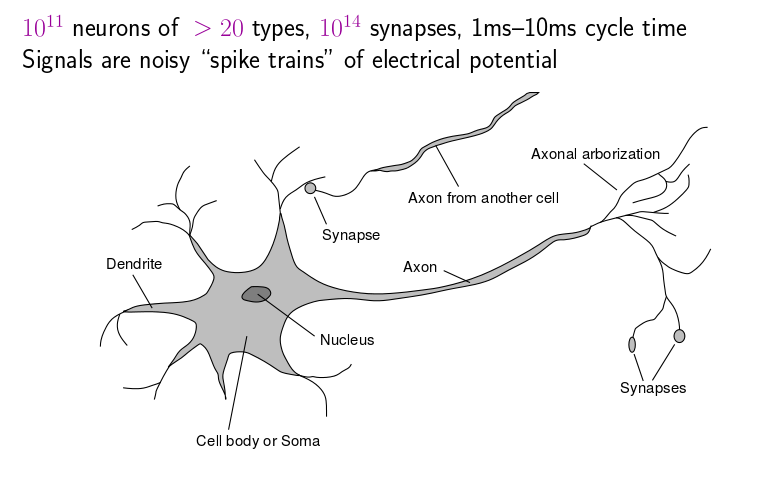
\includegraphics[scale=0.4]{brains.png}
    \end{center}
\end{frame}
\begin{frame}{}
    \begin{center}
        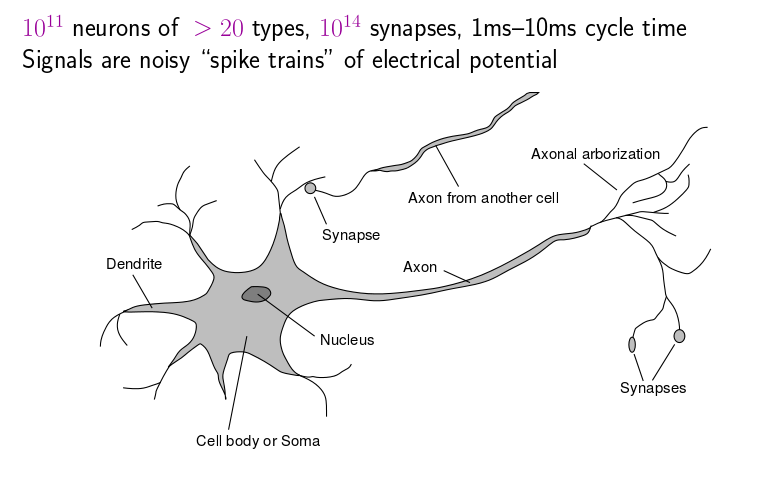
\includegraphics[scale=0.4]{brains.png}
    \end{center}
\end{frame}
\begin{frame}{}
    \begin{center}
        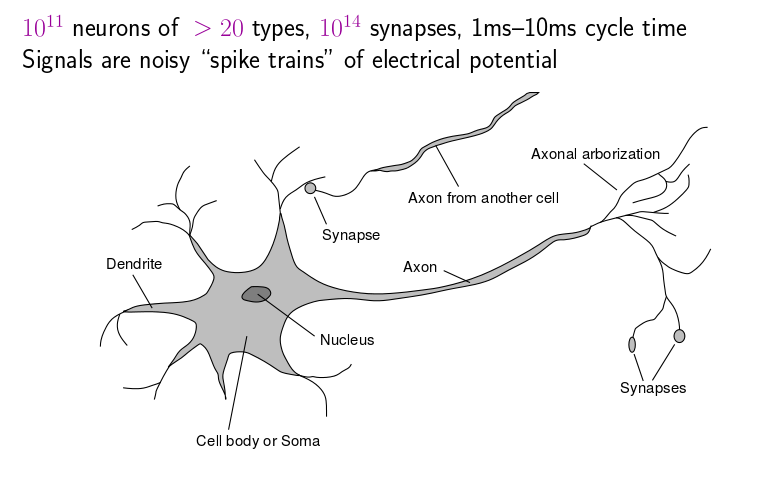
\includegraphics[scale=0.4]{brains.png}
    \end{center}
\end{frame}

\section{Summary}
\begin{frame}{Summary}

\tblue{Major Concepts:}
\begin{itemize}
    \item Probabilistic interpretation of Classification
    \item Bayesian Classifiers
    \item Naive Bayes Classifier
    \item Support Vector Machines (SVM)
    \item Kernels
\end{itemize}
\end{frame}

\begin{frame}{Slide Material References}
\begin{itemize}
    \item Slides from TSK Book, Chapter 5 
    \item Slides from Piyush Rai 
    \item See also the footnotes
\end{itemize}
\end{frame}


\end{document}

